\section{Softwarepaket}

die Allgemeine Idee ist die Industrialisierung eines Kompressores im 
Industrie 4.0.Die Sensoren liefern die Werten und diese Werten m"ussen 
von Arduino zu dem PC gelesen und geliefert.Um die Graphe zu erstellen,
wird PHP benutzt. Danach wird die Integrale berechnet.
Es wird auch SQL verwendet ,um die Daten zu speichern.

\subsection{Sensoren Auslesen}

Es werden im Programm Arduino alle Eing"ange den Sensoren und Variable defeniert.
Es wird 3 PT100 benutzt und jeder liefert 5 Werten f"ur 5 Cyclus das bedeutet 15 Werten. 
Drucksensor liefert 100 Werten bzw 500 Werten f"ur 5 Cyclus sowie den Dehnmessstreifen.
Aus diesem Grund wird es den Durschnitswert gemacht, um insgesamt 
203 werten zu bekommen.Die drei Interrupt die definiert sind, Signal A, Signal M und S.
Die Interruput S wird gemacht, weil man 5 Umdrehungen braucht. Signal 13 ist als Output definiert und schickt das Signal zu den Pin S,
damit diese Interruption funktionieren kann. Nachdem die Informationen bekommen wurden , m"ussen  diese Interuptionen deaktiviert werden.



\subsection{Sendung der Daten}

Um die Daten zu senden, es wird drei wichtigen Funktionen ben"otigt.Diese Funktionen sind Serial Beginn,
Serial Println und Baudrate.Die Funktion Serial Beginn() weist 
den Arduino an, eine serielle Verbindung mit 9600 bps herzustellen.
Mit der funktion Serial Println wurde die serielle Verbindung gesendet 
und pr"uft ,ob die daten von 3 Sensore der Temperature,Druck und Dehnmesstsreifen in PHP gezeigt werden .
Die Funktion Buadrate hat die gleiche Aufgabe wie Serial Beginn(). die geh"ort zu PHP 
und sie ist sehr wichtig , damit die Komminication zwischen PHP und Arduino richtig gemacht wird.
   
\subsection{Empfang der Daten}

Bei der Empfang der Daten sollte der serielle Port vom Arduino definiert werden. 
Danach wurde es ein Objekt Serielle erzeugt,damit der Empang der Daten gemacht wird.
Die fonction deviceOpen spielt eine wichtige Rolle, um die Daten zu empfangen.
Ohne diese Function k"onnte keine Kommunication angefangen werden. Da f"angt die
RX zu leuchten und das bedeutet der Start der Kommunication mit Arduino.
Bevor PHP eine Nachricht zu Arduino schickt ,ist es notwendig in diesem Fall eine Wartzeit zu machen, Weil PHP eine Wartezeit 
ben"otigt, um die Daten zu lesen, denn Arduino braucht Zeit , um die Werten zu schicken.
Die Werten, die von PHP gelesen werden sind 203 Werten ,3werten von 
den Temperatursensoren ,100 Werten von Drucksensoren und 100 Werten von Dehnmessstreifen.
Diese Werten werden im Serielle Communication gespeichert und dann werden
 diese Werten Zeileweise gelesen,daf"ur wird die Funktion ReadMessageByLine verwendet.
Die Werten werden danach als Ergebnis in einem Tabelle gespeicht werden.
Nach dem alle Werten gelesen sind, schlie"st die Funktion deviceopen den seriellen Port,d.h die Kommunication ist abgeschlossen.


\subsection{Verarbeitung der Daten in PHP}

Im programm PHP werden die Werten von Temperatursensoren,Drucksensor und 
Dehnmessstreifen umgewandelt. Bei den Temperatursensoren müssen die Temperatuspannungen umgewandelt,
damit man an Ende die Werten in Celisius bekommt.Dafür müssen die Widerstände der Temperatursensoren berechnet werden.
Um die zu berechnen , wird diese Gleichung benutzt:

\begin{equation}\label{eq:paran}
 Rt = av + b
\end{equation}
 F"ur die Berechnung der Wert A wird diese Gleichung benutzt:
 
\begin{equation}\label{eq:paran}
 a = \frac{Rmax-Rmin}{Vsmax-Vsmin}
\end{equation}

B ist der minimale Widerstand und es wird die Wert 91bei V=0 benutzt.
Danach werden Vsmax und Vsmin berechnet.

\begin{equation}\label{eq:paran}
 Vsmax = Vb(+) - Vb(-)
\end{equation}

\begin{equation}\label{eq:paran}
 Vb(+) = V\frac{Rt}{Rt+R} =24 \frac{200}{200+3300} = 1,37 V
\end{equation}

\begin{equation}\label{eq:paran}
 Vb(-) = V\frac{Rt}{Rt+R} =24 \frac{91}{91+3300} = 0,64 V
\end{equation}

\begin{equation}\label{eq:paran}
 Vsmax = Vb(+) - Vb(-) =1,37 -0,64= 0,73 V
\end{equation}

Nach der Berechnung wurde es festgestellt dass die Werte von Vsmax zu klein ist. 
Aus diesem Grund muss ein Operationelverstärker benutzt werden.
Laut der Gleichung der Operationelverstärker wird Vsmax neu berechnet mit dieser Formel wie folgt.

\begin{equation}\label{eq:paran}
 Vsmax = \frac{R7}{R8+R4}(Vb(+)-Vb(-)) =\frac{47000}{270+6800}(0,73) = 4,85 V
\end{equation}


\begin{equation}\label{eq:paran}
 Vsmin =  Vb(+) - Vb(-)
\end{equation}

\begin{equation}\label{eq:paran}
 Vb(+) = V\frac{Rt}{Rt+R} =24\frac{91}{91+3300}=0,64
\end{equation}


\begin{equation}\label{eq:paran}
 Vb(-) = V\frac{Rt}{Rt+R} =24\frac{91}{91+3300}=0,64
\end{equation}

laut der Berechnung Vsmin=0 und schlie"st sind alle Werten Berechnet ,um die Wert von a zu bekommen 

\begin{equation}\label{eq:paran}
a = \frac{200-91}{4,85} =22,47
\end{equation}
Wenn die Rt berechnet ist, k"onnte die Temperatur zu Celisius laut dieser Formelsatz umgewandelt werden.

\begin{equation}\label{eq:paran}
T = \frac{Rt -R0}{R0.\alpha}
\end{equation}

Bei der Drucksensor wurde es  auch ein Paar Berechnungen gemacht um die 
Werten zu Konvertieren.Damit der Graph(P,V) erstellt werden k"onnte. 
Der Drucksensor ist linear ,deshalb wird die Methode der Dreisatz gemacht ,um den Ausgangsstrom zu Bar konvertieren.
\begin{equation}\label{eq:paran}
Druck\underline{\ }Voltage = \frac{Druck\underline{\ }Ergebnis}{1023}.5
\end{equation}

Laut der folgenden Gleicheung wird der Strom berechnet.
\begin{equation}\label{eq:paran}
U = R.I 
\end{equation}
Wenn der Strom berechnet ist ,musste zu bar umgewandelt sein. Der Drucksensor funktioniert im Bereich [0,16],
deshalb wird die wert 16 bei der Umwandlung genutzt.
\begin{equation}\label{eq:paran}
Konvertiertdruck =\frac{Druck\underline{\ }I*16}{20*10^{-3}}
\end{equation}

Die Werten der DMS m"ussen auch konvertiert werden. Mit den konvertierten 
Werten konnte das Diagramm der Moment erstellt werden.
In diesem Fall werden noch \(\epsilon \), \(\sigma \) und der Moment berechnet werden.

\begin{equation}\label{eq:paran}
DMS\underline{\ }Voltage = \frac{DMS\underline{\ }Ergebnis}{1023}.5
\end{equation}

\begin{equation}\label{eq:paran}
\epsilon  = \frac{DMS\underline{\ }Voltage}{K.DMS\underline{\ }Vs.100}
\end{equation}

\begin{equation}\label{eq:paran}
\sigma  = E*\epsilon
\end{equation}


\begin{equation}\label{eq:paran}
Moment = \frac{\sigma*10^9*DMS\underline{\ }Igz}{DMS\underline{\ }Ymax}
\end{equation}


Der Berechnete Moment ist die Konvertierte Werte der DMS und mit diesen Werten ,könnte das Graph erstellt werden.
Alle diese Berechnungen werden in PHP gemacht, weil Arduino nicht in der Lage ist, alle diese Berechnungen zu machen.

Die Abbildung~\ref{fig:Orga} zeigt das Organigramm, das die Arbeit von PHP erkl"art

\begin{figure}[!htb]
\begin{center}
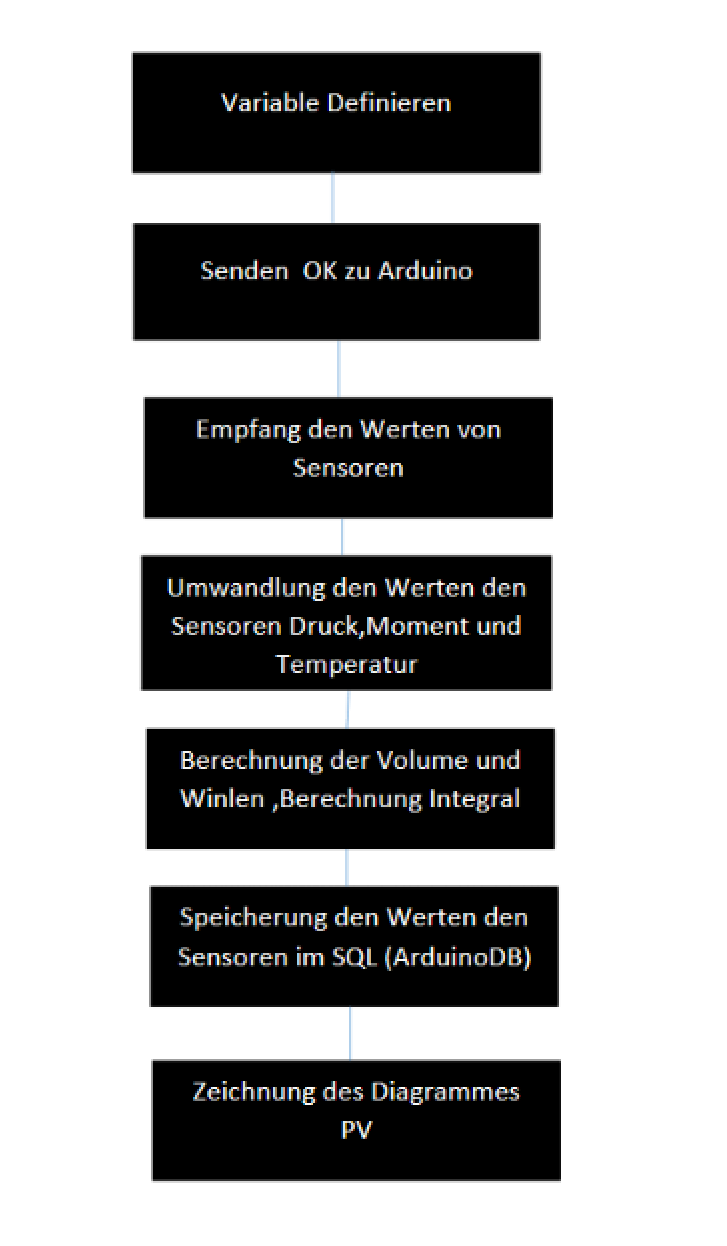
\includegraphics[height=20cm]{bilder/Orga.eps}
\end{center}
\caption{Organigramm PHP}\label{fig:Orga}
\end{figure}


\begin{figure}[!htb]
\begin{center}
\includegraphics[height=25cm]{bilder/or.eps}
\end{center}
\caption{Organigramm Arduino}\label{fig:Orga}
\end{figure}

